\chapter{Project Goals and Technologies}
\label{chap:intro}


\section{Introduction}
\begin{flushleft}
	This report's structure will follow this style:
	\begin{itemize}
		\item First: The report will outline the project's goals, the system architecture and the technologies used.
		\item Second: The report will detail the implementation of the varies system components from the start to the working prototype.
		\item Third: The report will outline the challenges faced in the implementation of the system.
		\item Fourth: A conclusion will be given including both technical and personal reflection along with detailed analysis on proposed work to be completed in
		      semester two.
	\end{itemize}
	\subsection{Motivation}
	I will use this project as a vehicle to explore and test both industry standard and brand-new technologies with an emphasis on open-source tech. This will stress test my knowledge of the
	technologies and both allow me to see what I can implement along with being a showcase of my skills in the field to potential employers. \newline
	The motivation for this project comes from the major pain points of mine, from my previous career as a bar owner and manager. \\ This project focuses on building a system for use by 
	bar/ public houses(pubs) and as such a single bar entity will be referred to as a \emph{user} of the system.\\
	There is also scope for this system to be altered slightly and to be used with any business which follows a similar back-end structure.
	\bigbreak
	Some of the most time-consuming and least valuable, from a time - reward perspective, are the back-end processes of running the business. I'm defining reward here as the actions which result
	in potential business growth. Time spent scanning invoices from suppliers, filling out income and expenditure spreadsheets and calculating gross and net figures(which I will refer to 
	as ‘\emph{group A}’ activities), whilst these processes are critical to a business’ operation and regulatory compliance - do not do much for business growth. 
	On the other hand, time spent on sourcing new products/ inventory, finding new/ novel forms of entertainment, business promotion and customer engagement(which I will refer to as 
	‘\emph{group B}’ activities) are the catalysts which drive sales and business growth.
	\bigbreak
	I hypothesize that this should lead to a healthier and more innovative industry by virtue of the extra amount of time spent on group B activities. With implementation of this system,
	barriers to entry should be broken down which should only help to increase innovation. This comes from the new entrants into the industry who may excel in group B processes but do not have 
	the knowledge or the confidence in their ability to perform the group A processes at a satisfactory standard. If these processes are automated then there should be fewer barriers of entry.
	Furthermore, the implementation of this system should increase the quality of life of business owners who no longer have to carry out manual data entry and monotonous 
	The aim is to provide more time for group B growth activities and processes by automating the group A processes in this project. For this to be accomplished there is a list of processes that 
	need to be tackled. \\ These processes fall into two broad categories, namely:
	\begin{itemize}
		\item The first category comes from the data collected from a sale of a users' product(a pub selling a beverage)
		\item The second stems from the data collected from a users purchases in relation to inventory.
		\end{itemize}
	These include:
	\begin{itemize}
		\item Keeping a record of all sale transactions that enter the system which will allow for the processing of sales, this is done by saving each transaction’s data to it’s own database
		\item The subsequent saving and updating of the transaction sales figures i.e. gross, net figures to their own database
		\item The updating of the inventory levels of products per sale
		\item The scanning of supplier invoices and key information extraction from the invoices
		\begin{itemize}
			      \item Updating of inventory levels as stock is delivered/ invoiced
			      \item Updating of cash flow levels
		      \end{itemize}
	\end{itemize}

	This is quite a lengthy list of processes to implement. It can be broken into two main components. 

	 For this FYP I will be simulating the Point of Sale(PoS) till software with fake data as I do not have time to build a user facing PoS system.
	If time constraints allow, I would like to incorporate transactional data from a current free and popular PoS application. This will most likely be SquareUp PoS by Square as my business uses this PoS currently and there is a developer API which can potentially be leveraged to provide the transactional data into the system. This is more of a “want” currently.

	There are many useful features which become available as a result of having all of this information available in one system. These insights come in the form of individual data per business but also trends and such from the data aggregated from users of the system. Some of these include:

	The ability to do some exploratory data analysis and other ML activities which can provide the businesses that use the system with some new data driven insights about the business. These insights would usually only be available to larger businesses with IT teams or businesses with owners who are data science savvy. Businesses with these characteristics in the drinks industry make up only a tiny fraction of the population based on my decade plus of experience within the industry and questions I have posed to other business owners/ management.

	An example of some more insights that can be derived from the information in the system, given decent levels of adoption in the industry, are live sales per product. Having a multitude of different businesses using the system, the sales of specific items can be accessed in real time. This provides some invaluable data to brewers of sales which can be utilised to precisely schedule production times and quantities.

	Further motivation
	The system I am building is an amalgamation of numerous different concepts and modules that I have studied over the past 4 years. I am using this project as a way to try and implement some of the architectures, processes and technologies that are industry standard and at the cutting edge of innovation in the tech industry. These include: (maybe go into detail on each one here)
	Event-driven Micro-service architecture
	Kubernetes
	Apache Kafka
	Debezium Change data capture
	Deep learning Neural Networks
	\bigbreak
	The motivation for this research paper is to explore some technologies that would build a cloud native build a \emph{cloud native} system that
	is highly scalable and as efficient as possible with as much of the processes automated as can be done.\newline
	A system that is capable of reacting - in real time - to changes i.e. any of the CRUD operations in a database. \newline
	Upon these change events occurring, the changes to the data in the system which triggered the events should be made
	available to other services/ components of the system to allow for the business logic, processing of data and subsequently
	business goals of the system to be met.
	To aid with accomplishing these requirements the system design is of an event-driven, microservice architectured nature.
	\newline
	\subsection{High Level Architecture}
	Debezium will be looking after the change events from a PostGres database, interacting with and utilizing Apache Kafka \autocite{ApacheKafka} for the event streams.
	The deployment orchestration is managed by Kubernetes, in this case I'll be using a single Kubernetes node on my machine by utilizing Minikube\autocite{MinikubeStart}.
	These are the primary technologies around which this term paper will focus.

	\subsection{System Goals}
	The goals for this system are to:
	\begin{itemize}
		\item Utilize an API which exposes an endpoint external to the Kubernetes cluster.
		\item Once that endpoint is hit, the API creates some data which is saved to a database.
		\item Configure the Debezium PostGres connector to listen for changes in the state of the database. Debezium will then utilize Kafka Connect to ingest the stream updates,
		      those updates are then pushed to Kafka Topics.
		\item Create a consumer which is subscribed to a Kafka Topic to consume the changes and prove the system is operating nominally.
		\item Automate as much of the processes as possible.
		\item Focus on the use of open source technologies.
	\end{itemize}
	\subsection{System Architecture}
	The following is the system architecture diagram:
	\begin{figure}[ht]
		\begin{center}
			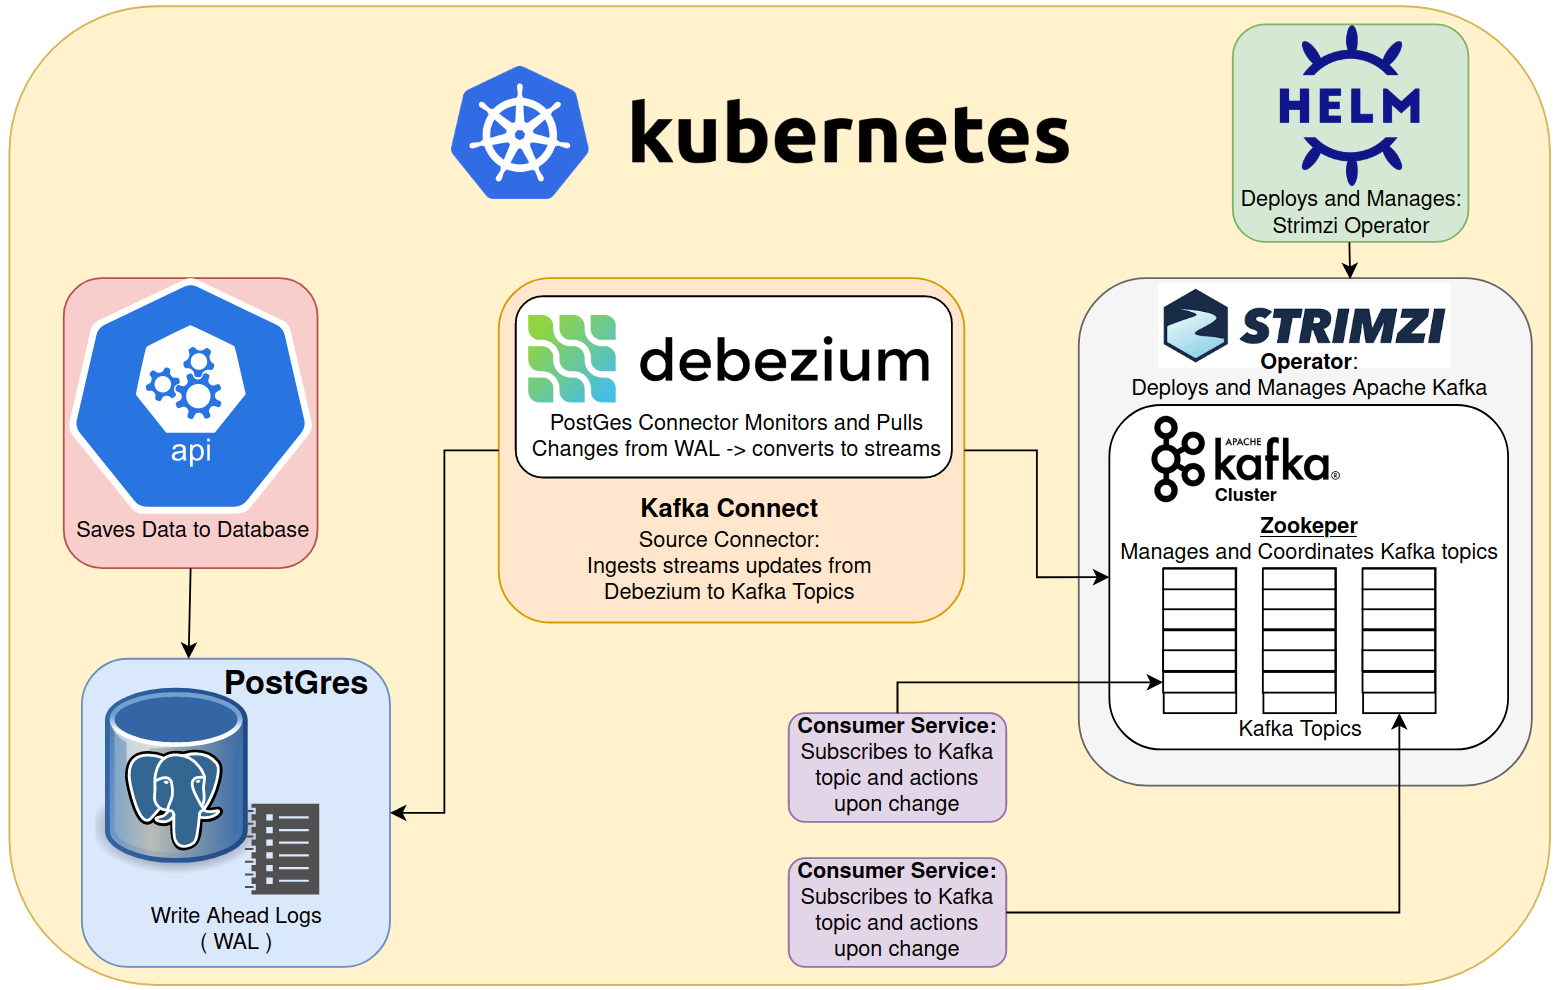
\includegraphics[width=1\textwidth]{figures/architecture_v2.png}
			\caption{Architecture of the system depicting the interaction between components.}
			\label{fig: 1.1}
		\end{center}
	\end{figure}
	\bigbreak
	\textbf{Note:} The system architecture has a section that is not 100\% accurate. Strimzi deploys and manages the Kafka Connect component, via a deployment manifest,
	and the initial diagram was implemented as such. However, since Debezium is implemented on top of Kafka Connect but not deployed by or managed by Strimzi, the decision
	was taken to remove the Kafka Connect component	from the Strimzi component for better clarity, with this explanation in place to address questions.
	\bigbreak
	All the black arrows in the diagram do not depict a flow of data through the system. They are a representation of the interactions between
	components. As an example:\newline The arrow from \textbf{Helm}	to \textbf{Strimzi} represents the deployment of the Strimzi operator component by the
	Helm package manager.
	\section{Technologies Used}
	\subsection{Kubernetes}
	Kubernetes is an open-source container-orchestration system for automating computer application deployment, scaling, and management. It was originally designed
	by Google and is now maintained by the Cloud Native Computing Foundation(CNCF) \autocite{ProductionGradeContainerOrchestration}. A whole paper could be written about Kubernetes,
	but for the sake of brevity this report will only explain Kubernetes components explicitly relevant to this project. This report utilizes Kubernetes for orchestration,
	deployment and fault-tolerance.
	\newline Fault-tolerance is taken care of by Kubernetes as Kubernetes routinely compares pods and services currently active/ healthy and restarts the pods
	which have deviated from the desired configurations or found themselves in an `unhealthy' state.\newline
	Kubernetes' services are deployed in a cluster via a deployment manifest. The deployment manifest is either a JSON file or a YAML file which describes the desired state
	of the service. The Kubernetes control loop is responsible for monitoring the state of the cluster and making changes as necessary. If a service is not running or has drifted
	from the desired state, the control loop restart the service from the deployment manifest.
	\bigbreak
	Most other Kubernetes resources are created in the same manner and are \emph{applied} to the cluster using \code{kubectl}. Kubectl is a command line tool which is used to
	interact with the Kubernetes cluster. Resources are applied using the \code{apply} command. \code{kubectl apply -f \emph{resource-manifest-file-name}} is used to apply a resource to the cluster. \newline
	This paper will also use \textbf{Helm} which is Kubernetes' package manager\autocite{UsingHelm}.
	\subsection{API for System Data}
	Since this report will focus on capturing changes from a database, there will need to be a methodology for creation and saving the data.
	This is handled by an API in current development. It is essentially a Transaction API, it exposes an endpoint and which creates a fake transaction. This
	transaction is a typical transaction that would be found in a pub/ bar. It has a transaction owner, this is the entity for which the transaction has been
	possessed, in this case a pub/ bar. The transaction contains a random number of beers with some randomized information for things like name, ABV,
	price etc. The API is written in GoLang and uses Gorilla Mux(a high performance HTTP router package).
	\subsection{Debezium}
	Debezium is an open source Change Data Capture (CDC) technology which is configurable with a number of different connectors. There are specific connectors for each of the supported databases.
	PostGres, MySQL and MongoDB are some of the supported databases \autocite{ConnectorsDebeziumDocumentation}.\newline
	Debezium is most commonly deployed via Apache Kafka's Kafka Connect framework \autocite{KafkaConnectConfluent}. Once a Debezium connector is applied to continuously monitor a database, it ingests the changes and then
	utilizes the Kafka Connect component to push the changes to Apache Kafka topics. It lets any of your applications/ services stream every-row level change whilst preserving the order by which
	the changes were committed to the database \autocite{debeziumcommunityDebezium}. In the case of Postgres, it does this by monitoring Postgres' \emph{Write Ahead Logs}. These are binary logs
	of every event to the database. These include not only all CRUD updates to the database but schemas along with schema modifications also.
	\bigbreak
	Debezium may also be deployed via the Debezium server \autocite{DebeziumArchitectureDebezium}. This is a ready-to-use application which streams changes to a variety of different messaging systems including Redis, AWS Kinesis, Google Pub/Sub,
	and more.
	\bigbreak
	There are some great reasons to use Debezium. It is an extremely efficient way to capture changes to a database because of the way it utilizes the WAL, Debezium can process changes in the database without having to
	interact with the database via the usual methodologies of expensive	database calls i.e. SELECT, INSERT etc. \newline
	The conversion of these changes to streams can allow for multiple services to access the data changes relevant to them without having to interact with the database, so the database' primary job
	becomes servicing the incoming requests from the API.
	\bigbreak
	This report will utilize Debezium's Kafka Connect implementation along with the aforementioned Postgres connector.
	\subsection{Apache Kafka}
	Apache Kafka is a high performance, distributed, fault-tolerant, event streaming broker/ event bus. It was originally developed at LinkedIn but was open sourced in 2011 and is now maintained by the
	Apache Software Foundation. It is currently in use in more than 80\% of all Fortune 100 companies.\newline
	Event streaming is the process of capturing live events such as a CRUD operation to a database or other data
	from services. These services can be applications of any type. Mobile apps, web applications, microservices, IoT devices, etc. \newline
	According to Kafka documentation \autocite{ApacheKafka}, it combines three key capabilities, namely:
	\begin{itemize}
		\item To allow publishers to write and subscribers to read streams of events, including continuous import/export of data from other systems.
		\item To store streams of events durably, reliably and in a fault-tolerant replicated manner.
		\item To process streams of events in real time or retrospectively as desired.
	\end{itemize}
	Kafka can be simply thought of as a distributed system which consists of servers and clients. Kafka can span multiple nodes and be run anywhere. Communication between the two happens via the TCP protocol.
	\begin{itemize}
		\item \emph{Servers}: The servers that make up the storage layer of the system are called \textbf{brokers}. These brokers save events to topics. These topics are like logs, brokers append the events
		      to the topic and consumers read from the topic via an offset. This ensures that the topics are read in order. Topics may be partitioned and replicated across multiple brokers. This ensures
		      fault-tolerance and durability. Events can be read by a multitude of consumers and are kept for any configurable amount of time. \newline
		      Other servers run \textbf{Kafka Connect} which handles the continuous import and export of data as event streams to the topics.
		\item \emph{Clients}: The clients that make up the application layer of the system are called consumers. These consumers read from topics and process the events. This can be done in parallel and
		      as such can be used to process data at large scale.
	\end{itemize}
	Apache Zookeeper manages and coordinates the brokers. Kafka uses it to ensure data durability. If a leader node/broker fails, Zookeeper ensures a new leader is
	chosen without any consequence to data in the system via a leader election. It is a highly scalable, high-availability, distributed coordination system \autocite{WhatZookeeperWhy}.
	\begin{figure}[ht]
		\begin{center}
			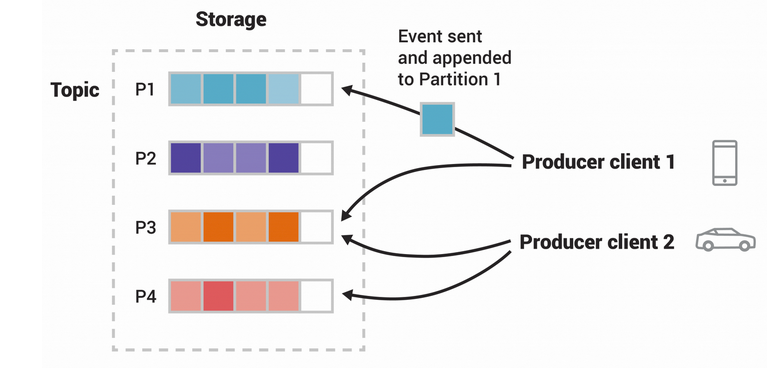
\includegraphics[width=.7\textwidth]{figures/topics.png}
			\caption{Simplified view of a partitioned topic being written to by multiple producers\autocite{ApacheKafka}. In this report there will be just one producer, the Debezium Kafka Connect instance.}
			\label{fig: 1.2}
		\end{center}
	\end{figure}
	\pagebreak
	\subsection{The Strimzi Operator}
	Strimzi is an open-source Kubernetes operator that deploys Apache Kafka in a Kubernetes cluster using the operator pattern. \newline
	Operators are extensions to Kubernetes that are deployed using a \emph{Custom Resource Definition} (CRD). A Kubernetes operator is a method of packaging, deploying and
	managing a Kubernetes application \autocite{WhatKubernetesOperator}. Operators are essentially just a non Kubernetes-native piece of software that extends the functionality of Kubernetes.
	Operators follow the Kubernetes control	loop and other Kubernetes principals. An operator can be thought of as a client of the Kubernetes API that acts as a controller
	for a Custom Resource \autocite{OperatorPattern}. Their goal is to bring the Kubernetes core concept of automation to non-Kubernetes components but with the added elements
	of domain/ application-specific knowledge about the application it deploys via its own set of preconfigured and configurable CRDs that are specific to the application it deploys.
	Operators aim to automate the entire life cycle of the software under their control.
	\begin{figure}[ht]
		\begin{center}
			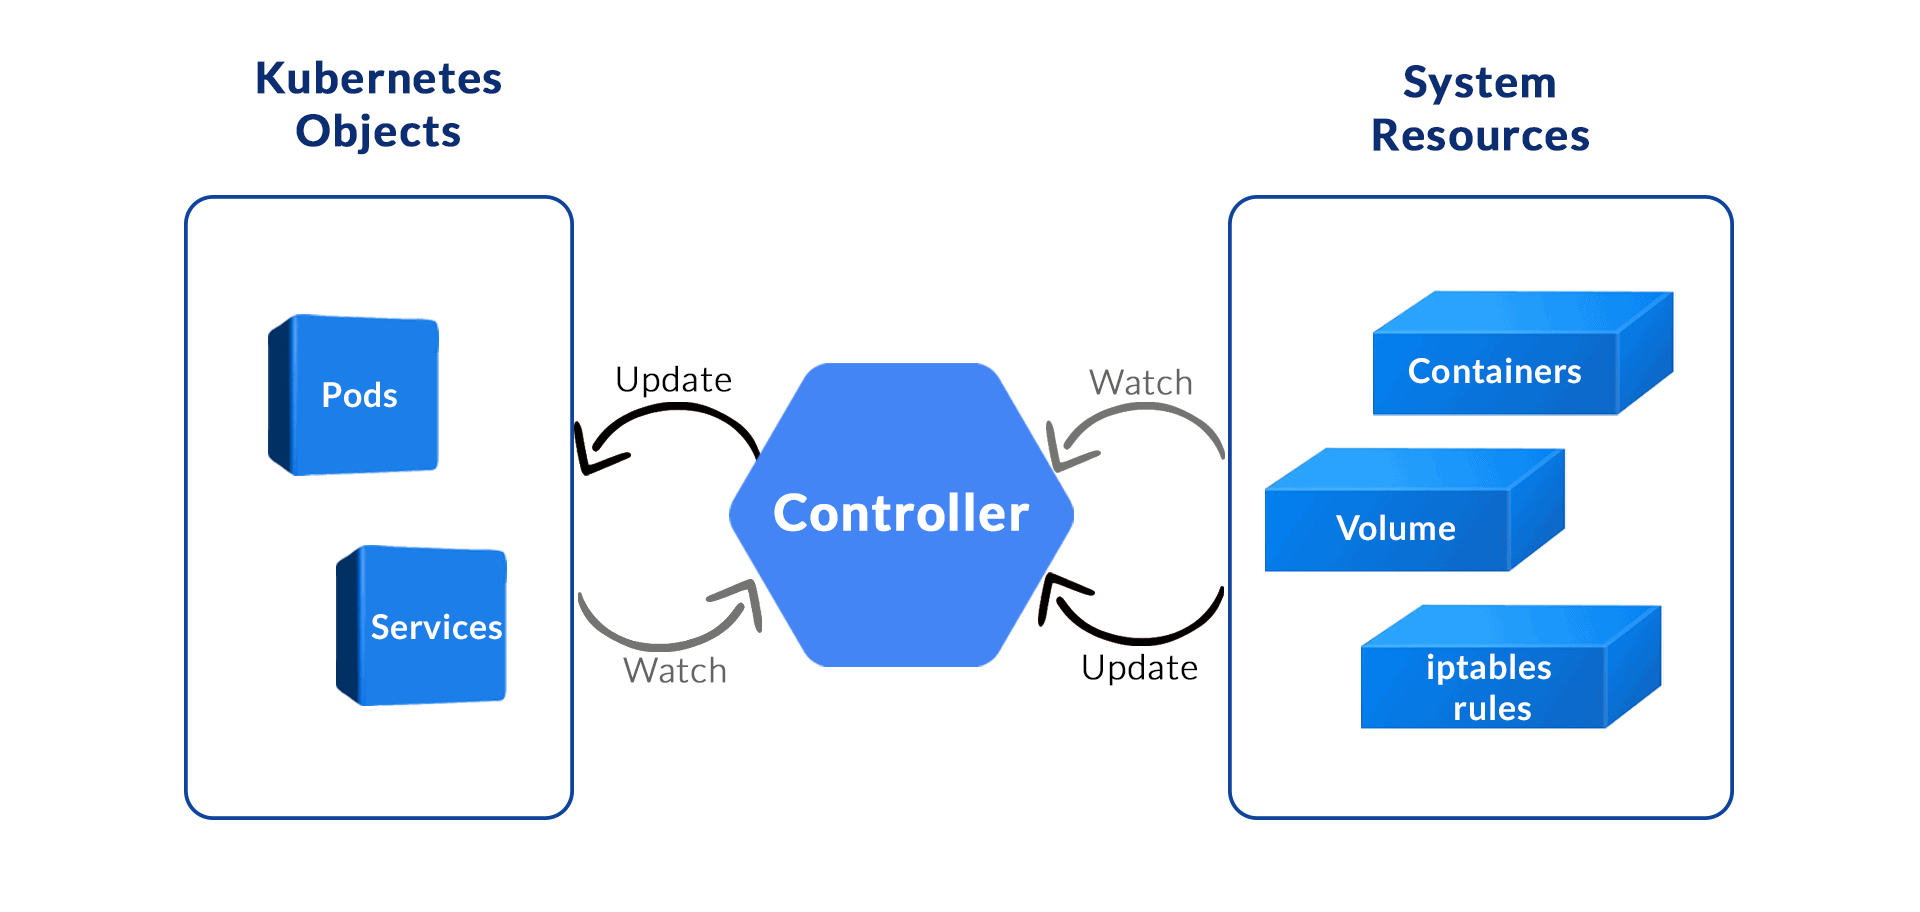
\includegraphics[width=.8\textwidth]{figures/operator_control_loop.png}
			\caption{Operator control loop based on the Kubernetes \emph{Observe, Act, Analyze} control loop. Sourced from \autocite{KubernetesOperatorStateful2021}.}
			\label{fig: 1.3}
		\end{center}
	\end{figure}
	\pagebreak
\end{flushleft}
